\liitetyyli
    \section{Lähtötasotesti}
% vastaukset voisi olla jossain takana eikä tässä ettei kovin moni lukisi niitä ennen testiä

% FIXME: On mietittävä, mikä on lähtötasotestin tarkoitus. Tarvitaanko sitä tässä oppikirjassa vai ei. Luultavasti voisi poistaa. Onko sen teettäminen järkevää ajankäyttöä? Mikä on sen rooli? Kannustava alkuverryttely, opettajalle koko vuosiluokan tarkasteluun työkalu vai jotain muuta?
% no ei se negatiivista voi olla, että tämä on. Käyttäkööt, jos käyttävät. Hommas selvä. –Joonas%

\subsection*{Lähtötasotesti kurssille MAA1}

% FIXME: Muokataan tehtäväympäristöä niin, etteivät nämä jatka vanhaa tehtävänumerointia.
\begin{tehtava}
Laske. Merkitse välivaiheet näkyviin. 
\begin{enumerate}
\item $2+3\cdot 2-1\cdot5$
\item $(2+1)^2+\frac{4-2}{2}$
\end{enumerate}
\begin{vastaus}
\item $2+6-5=3$
\item $3^2+\frac{2}{2}=9+1=10$
\end{vastaus}
\end{tehtava}

\begin{tehtava}
Laske. Merkitse välivaiheet näkyviin. 
\begin{enumerate}
\item $4\cdot \frac{2}{5} + \frac{2}{3}\cdot \frac{3}{5}$
\item $\frac{2}{5} : \frac{3}{2}$
\end{enumerate}
\begin{vastaus}
\item $\frac{8}{5} + \frac{2}{5}=\frac{10}{5} = 2$
\item $\frac{2}{5} \cdot \frac{2}{3}=\frac{4}{15}=$
\end{vastaus}
\end{tehtava}

\begin{tehtava}
\begin{enumerate}
\item Kuinka paljon on 5~\% luvusta 40?
\item Kuinka monta prosenttia 2 on luvusta 4?
\end{enumerate}
\begin{vastaus}
\item 2
\item 50~\%
\end{vastaus}
\end{tehtava}

\begin{tehtava}
Sievennä.
\begin{enumerate}
\item $x + 2x+x^2$
\item $2(4x+1)$
\end{enumerate}
\begin{vastaus}
\item $2x +x^2$
\item $8x+2$
\end{vastaus}
\end{tehtava}

\begin{tehtava}
\begin{enumerate}
\item Matka ja aika ovat suoraan verrannollisia. Jos matka kaksinkertaistuu, niin miten käy ajalle?
\item Sievennä $-3x+4x^2-2x+x^2$.
\end{enumerate}
\begin{vastaus}
\item Aika kaksinkertaistuu
\item $5x^2-5x$
\end{vastaus}
\end{tehtava}

\begin{tehtava}
Ratkaise yhtälöt.
\begin{enumerate}
\item $2x+5 = -1$
\item $x^2 = 9$
\end{enumerate}
\begin{vastaus}
\item $x=-3$
\item $x=-3$ tai $x=3$
\end{vastaus}
\end{tehtava}

\begin{tehtava}
Funktiot on määritelty seuraavasti: $f(x)= x^2+3x$ ja $g(x)=2x-8$.
\begin{enumerate}
\item Laske $f(-2)$.
\item Millä $x$:n arvolla $g(x)=0$?
\end{enumerate}
\begin{vastaus}
\item $(-2)^2+3\cdot(-2)=-2$
\item $x=4$
\end{vastaus}
\end{tehtava}


    \chapter{Numerot ja luvut}

Ihmisillä ja eläimillä on luonnostaan matemaattisia taitoja. Monet niistä, esimerkiksi lukumäärien laskeminen, ovat monimutkaisia ajatusprosesseja, jotka kehittyvät lapsuudessa – toisilla aiemmin, toisilla myöhemmin. Koulussa opeteltava peruslaskento ja myös matematiikka tieteenalana rakentuvat tämän biologisen osaamisen päälle. Laskeminen itsessään on vain eräs matematiikan osa-alue, eikä kaikki matematiikka ole laskemista.

% vanha sivulaatikko
\laatikko{Huom.! Count (engl.) = 'laskea lukumäärä'. \\ Calculate (engl.) = 'tehdä laskutoimitus'. }

\subsubsection*{Yleisesti lukujen merkitsemisestä}

% Laskutoimitusten ja muun matemaattisen pohdinnan merkitseminen kirjalliseen muotoon on taito, jonka oppiminen oli merkittävä askel ihmisen kehityshistoriassa.
Ihmisen kehityshistoriassa tapahtui huomattava askel, kun laskutoimitukset ja muu matemaattinen pohdinta opittiin merkitsemään kirjalliseen muotoon. Aikojen saatossa eri kansat ovat käyttäneet erilaisia tapoja merkitä laskutoimituksia ja lukumääriä. Tunnettu esimerkki on roomalaiset numerot, jotka näyttävät hyvin erilaisilta nykyään käyttämiimme lukumerkintöihin.

Helpoin ja yksinkertaisin tapa merkitä lukumäärää on käyttää vain yhtä merkkiä ja toistaa sitä:

%\missingfigure{Piirrettynä ''tukkimiehen kirjanpitoa'' ja  vertaus arabialaisilla numeroilla}

\begin{center}
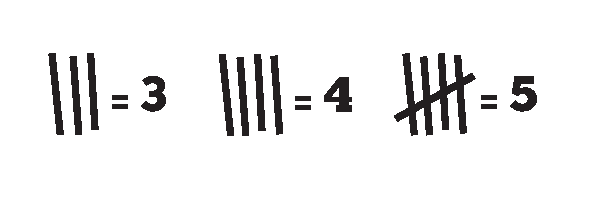
\includegraphics{pictures/Kuva1-1-tukkimiehenkirjanpito.pdf}
\end{center}

Kun käytettävissä olevien merkkien määrää lisää, suuria lukuja voi kirjoittaa lyhyempään muotoon. Tilanne on verrattavissa vaikkapa kiinan kieleen, jossa on käytössä satoja erilaisia kirjoitusmerkkejä. Merkeissä on paljon muistettavaa, mutta toisaalta kokonaisen lauseen voi kirjoittaa vain parilla kirjoitusmerkillä.



%%%ROOMALAISET LUVUT%%%%%%

\subsection*{Roomalaiset luvut}
Antiikin Roomassa käytössä olivat numeromerkit I, V, X, L, C, D ja M. Niiden numeroiden vastaavuudet meidän käyttämiimme lukuarvoihin ovat seuraavat:

\begin{equation*}
\rm I=1\quad
V=5\quad
X=10\quad
L=50\quad
C=100\quad
D=500\quad
M=1~000
\end{equation*}

%Huomaa, että suuri osa roomalaisista numeromerkeistä ovat jo itsessään arvoltaan niin suuria, että tarvitsemme niiden nykyilmaisuun monta merkkiä! Nollaa roomalaisissa numeroissa ei ole, ja tiettävästi tuhatta suurempia arvoja esittäviä numeromerkkejä merkkejä otettiin käyttöön vasta keskiajalla. 

Lukuja koostetaan näistä merkeistä siten, että merkit kirjoitetaan peräkkäin pääasiassa laskevassa järjestyksessä ja niiden numeroarvot lasketaan yhteen. Jos arvoltaan pienempi numeromerkki (korkeintaan yksi) edeltää suurempaa, pienempi vähennetään suuremmasta ennen yhteenlaskun jatkamista.

\begin{esimerkki}
$\text{XIV} = 10 + (5 - 1) = 14$
\end{esimerkki}

Roomalaisia numeroita käytetään usein myös nykyään merkitsemään esimerkiksi järjestystä.

\subsection*{Paikkajärjestelmä}

Kun numeroista koostetaan lukuja, numeroiden kirjoitusjärjestyksellä on väliä. Esimerkiksi luvut $134$ ja $413$ eivät ole sama luku; saamme eri lukuja, kun numeroita yhdistellään eri tavoin. Käsityksiä siitä, miten numeron paikka vaikuttaa luvun suuruuteen kutsutaan \emph{paikkajärjestelmiksi}.

Seuraava esimerkki selventää, miten roomalaiset muodostivat erilaisia lukuja numeromerkeistään.

\begin{esimerkki}
\ % Quick-and-dirty-fiksaus, kun ensimmäinen itemi meni ''Esimerkki.'' -tekstin perään
\begin{itemize} % https://github.com/sliedes/oppikirjamaraton-maa1/commit/e41c1cc6856f0f0b705e94b03378a1edd30f56d3
\item III$=1+1+1=3$
\item IX$=10-1=9$
\item XII$=10+1+1=12$
\item XIX$=10+(10-1)=19$
\item CDX$=500-100+10=410$
\item MDC$=1 000+500+100=1~600$
\end{itemize}
\end{esimerkki}
% Fiksattu sliedes:n kommentti: annettu kuvaus ja seuraava esimerkki itse asiassa on väärin;
% V:tä, L:ää ja D:tä ei koskaan vähennetä. Luku 1600 esitetään MDC.
% Ainakin yleisimmässä tavassa käyttää roomalaisia numeroita. 

\laatikko{Länsimaisessa traditiossa käytössämme on kymmenen numeromerkkiä: 0, 1, 2, 3, 4, 5, 6, 7, 8 ja 9. Näitä kutsutaan alkuperänsä mukaan hindu-arabialaisiksi numeroiksi.}

Kirjoittamalla näitä numeromerkkejä peräkkäin ilmaisemme lukuja.

% vanha sivulaatikko
\laatikko{Englannin kielen sana \textit{number} voi viitata sekä numeroon että lukuun. Sana \textit{digit} tarkoittaa pelkästään yhtä numeromerkkiä. Ruotsiksi luku on \textit{tal}, lukumäärä \textit{antal} ja numeroa tai lukumäärää tarkoittamatonta numeroyhdistelmää kuvaa suomen kielen tapaan sana \textit{nummer}.}

\begin{esimerkki}
Luku \[715531\] koostuu numeroista 7, 1, 5, 5, 3 ja 1.
Luku \[9\] koostuu ainoastaan vastaavasta numeromerkistä 9.
\end{esimerkki}

Luvulla on aina suuruus mutta numerolla ei. Tämän vuoksi esimerkiksi arkipäivän käsitteet postinumero ja puhelinnumero eivät ole lukuja, vaikka niissä numeroita yhdistelläänkin. Emme voi esimerkiksi sanoa, onko postinumero 00950 jollakin tapaa suurempi kuin postinumero 00900.

\subsection*{Lukujärjestelmät}

Järjestelmää, jolla merkitsemme lukuja kutsutaan \emph{kymmenjärjestelmäksi}. Siinä kunkin numeron paikka kertoo, kuinka monta kymmentä, sataa, tuhatta ja niin edelleen numero vastaa.

\begin{esimerkki}
Luku $562$ koostuu viidestä sadasta, kuudesta kymmenestä ja kahdesta ykkösestä, eli $562= 5 \cdot 100 + 6 \cdot 10 + 2$.

Luku $2~010,23$ koostuu kahdesta tuhannesta, yhdestä kymmenestä, kahdesta kymmenesosasta ja kolmesta sadasosasta. Desimaalimerkintöihin palataan tarkemmin Desimaaliluvut-osassa.
\end{esimerkki}

% vanha sivulaatikko
\laatikko{Kielioppihuomautuksia: 1) Tuhaterottimena käytetään välilyöntiä, ei pilkkua tai pistettä. 2) Suomessa on käytössä desimaalipilkku, ei -piste! Yhdysvaltalaiset ovat suunnitelleet laskimesi.}


Kymmenjärjestelmää kutsutaan myös \emph{desimaalijärjestelmäksi}, koska siinä hyödynnetään kymmentä eri numeromerkkiä. Muita yleisesti käytössä olevia järjestelmiä ovat 2-järjestelmä eli binäärijärjestelmä ja 16-järjestelmä eli heksadesimaalijärjestelmä, joita käytetään digitaalisen informaation tallentamiseen ja käsittelemiseen. Binäärijärjestelmässä luvun muodostavia numeromerkkejä kutsutaan biteiksi. Bitti voi olla joko päällä (1) tai pois päältä (0), ja toteutus tietokoneessa vastaa esimerkiksi sitä, että johtimessa kulkee virta (1) tai ei (0). Useampaa järjestelmää käytettäessä merkitään kantaluku luvun jälkeen alaindeksinä. Esimerkiksi luku yhdeksäntoista voidaan merkitä $19_{10}$, $10011_{2}$ tai $13_{16}$ käyttäen desimaali-, binääri- tai heksadesimaalijärjestelmää.

\begin{esimerkki}
\begin{align*}
19_{10} &= 1 \cdot 10 + 9 \\
10011_{2} &= 1 \cdot (2 \cdot 2 \cdot 2 \cdot 2) + 0 \cdot (2 \cdot 2 \cdot 2) + 0 \cdot (2 \cdot 2) + 1 \cdot 2 + 1 \\
13_{16} &= 1 \cdot 16 + 3
\end{align*}
\end{esimerkki}

Kuusitoistajärjestelmässä tarvitaan vielä kuusi uutta numeromerkkiä. Tavaksi on vakiintunut käyttää kirjainmerkkejä $\mathrm{A, B, C, D, E}$ ja $\mathrm{F}$. Ne vastaavat lukuja $10, 11, 12, 13, 14$ ja $15$. Yleisesti $n$-järjestelmässä käytetään $n$:ää kappaletta eri merkkejä, jotka merkitsevät lukuja nollasta lukuun $n-1$.

\begin{esimerkki}
$F4C_{16} = F \cdot (16 \cdot 16) + 4 \cdot 16 + C = 15 \cdot (16 \cdot 16) + 4 \cdot 16 + 12 = 3916_{10}$
\end{esimerkki}


\section{Kirjaimet symboleina luvuille}

''Jos tämä on kerran matematiikkaa, niin miksi käytätte kirjaimia?'' kysyy peruskoulun alaluokkien oppilas. Lyhyt vastaus on, että näin saamme yleistettyä monia tuloksia, eikä meidän tarvitse tutkia vain erikoistapauksia.

Numeroita kuvaavat merkit ovat mielivaltaisia symboleita. Lukujakin edustamaan päädytään joskus käyttämään jotakin lyhennysmerkintää, yleensä yksittäisiä latinalaisten aakkosten kirjaimia. Kenties yleisin mielivaltaista, tuntematonta lukua edustava symboli on kirjain $x$. Kulmien suuruuksia merkitään yleensä kreikkalaisilla kirjaimilla kuten $\alpha$ (alfa), $\beta$ (beeta) ja $\gamma$ (gamma).

Jos kaksi lukua $x$ ja $2$ ovat yhtä suuret, merkitään
$x=2$. Tällainen yhtäsuuruus pätee aivan hyvin myös toisin päin: $2=x$, joten kumpikin kirjoitustapa on tilanteesta riippumatta oikein. Jos luku $y$ on pienempi kuin $z$ merkitään $y<z$, tai toisaalta $z>y$.

% vanha sivulaatikko
\laatikko{Painotekstissä kirjaimella merkityt tuntemattomat ja muuttujat kirjoitetaan \textit{kursiivilla}. Sen sijaan aina saman arvon saavat tunnetut matemaattiset vakiot kuten $\uppi$ kirjoitetaan pystyyn.} %Painotekstissä kirjaimella merkityt tuntemattomat ja muuttujat kirjoitetaan \textit{kursiivilla} ja aina saman arvon saavat, tunnetut matemaattiset vakiot kuten $\uppi$ pystyyn.

Erilaisilla luvuilla voidaan suorittaa erilaisia laskutoimituksia. Seuraavissa luvuissa esitellään ja käydään läpi lukiomatematiikassa ja mahdollisissa jatko-opinnoissa käytettäviä lukujoukkoja ja tavallisimmat laskutoimitukset.

    \chapter{Yksiköt ja vastaustarkkuus}

\section*{Etuliitteet}

\laatikko{
Tavallisimmat kerrannaisyksiköiden etuliitteet:

\begin{tabular}{c|c}
\begin{tabular}{c|c|c}
Nimi & Kerroin & Tunnus \\
\hline
deka & $10^{1}$ & da 	\\
hehto & $10^{2}$ & h 	\\
kilo & $10^{3}$ & k 	\\
mega & $10^{6}$ & M 	\\
giga & $10^{9}$ & G		\\
tera & $10^{12}$ & T 	
\end{tabular}
\begin{tabular}{c|c|c}
Nimi & Kerroin & Tunnus \\
\hline
desi & $10^{-1}$ & d 	\\
sentti & $10^{-2}$ & c 	\\
milli & $10^{-3}$ & m	\\
mikro & $10^{-6}$ & $\upmu$ \\
nano & $10^{-9}$ & n 	\\
piko & $10^{-12}$ & p
\end{tabular}
\end{tabular}
}

Tietotekniikassa datan määrää mitataan tavuina, mutta siellä yksi kilotavu (kt) ei tarkoita tasan $1000$ tavua,  vaan $1024$ tavua ($2^{10}$). Vastaavasti yksi megatavu on $1024$ kt (eli $1048576 = 2^{20}$ tavua), yksi gigatavu $1024$ Mt jne.

\section*{Yksikkömuunnokset}

\laatikko{
Yksi tunti on $60$ minuuttia. Yksi minuutti on $60$ sekuntia.
\begin{itemize}
  \item $1~\text{h} = 60~\text{min}$
  \item $1~\text{min} = 60~\text{s}$
  \item $1~\text{h} = 60~\text{min} = 60 \cdot 60~\text{s} = 3600~\text{s}$ 
\end{itemize}
}

% FIXME \todo{taulukko amerikkalaisista yksiköistä}

\begin{esimerkki}
Kuinka monta minuuttia on $1,25$ h? $1,25 \text{h} = 1,25 \cdot 60 \text{min} = 75 \text{min}$. $1,35$ h on siis $75$ minuuttia. Huomaa, että voit laskuissasi esittää desimaaliluvun $1,25$ yhdistettynä lukuna $1 \frac{25}{100}$ eli $1 \frac{1}{4}$, mikä saattaa helpottaa laskemista.
\end{esimerkki}

\begin{esimerkki}
%\todo{esimerkki jossa tarvitsee ottaa huomioon kerrannaisyksikkö, esim. nanometri tai whatever.}
\begin{tehtava}
Muuta \emph{järkevimpään} yksikköön. \\
a) $0,3$ km + $200$ m \qquad
b) $0,04$ m + $10$ mm \\
c) $0,4$ km + $7000$ m + $1000000$ mm \\
d) $0,2$ cm + $4$ cm
\begin{vastaus}
a) $500$ m \qquad
b) $5$ cm \qquad
c) $8,4$ km \qquad
d) $4,2$ cm
\end{vastaus}
\end{tehtava}
\end{esimerkki}

\begin{esimerkki}
% FIXME \todo{esimerkki cm muuttamisesta tuumaksi ja toisinpäin}
% FIXME tämä pitäisi tekaista lukusuorana: \missingfigure{havainnollistava kuva, jossa on rinnastettu suoralla sentit ja tuumat}
\end{esimerkki}

\begin{tehtava}
Muuta minuuteiksi. \\
a) $1$ h $17$ min \qquad
b) $2$ h $45$ min \qquad
c) $1,5$ h \qquad
d) $1,75$ h
\begin{vastaus}
a) $77$ min \qquad
b) $165$ min \qquad
c) $90$ min \qquad
d) $105$ min
\end{vastaus}
\end{tehtava}

\begin{tehtava}
Muuta sekunneiksi. \\
a) $1$ h $42$ min \qquad
b) $3$ h $32$ min \qquad
c) $1,25$ h \qquad
d) $4,5$ h
\begin{vastaus}
a) $6120$ s \qquad
b) $12720$ s \qquad
c) $4500$ s \qquad
d) $16200$ s
\end{vastaus}
\end{tehtava}

\begin{tehtava}
Muuta tunneiksi ja minuuteiksi. \\
a) $125$ min \qquad
b) $667$ min \qquad
c) $120$ min \qquad
d) $194$ min
\begin{vastaus}
a) $2$ h $5$ min \qquad
b) $11$ h $7$ min \qquad
c) $2$ h \qquad
d) $3$ h $14$ min
\end{vastaus}
\end{tehtava}

% FIXME \todo{TEHTÄVÄ: muuta sekunneista tunneiksi, minuuteiksi ja sekunneiksi}
% FIXME \todo{TEHTÄVÄ: muuta minuuteista tunneiksi desimaalimuodossa, esim 1,25h}

\begin{tehtava}
Esitä luku ilman kymmenpotenssia. \\
a) $3,2 \cdot 10^4$ \qquad
b) $-7,03 \cdot 10^{-5}$ \qquad
c) $10,005 \cdot 10^{-2}$ \qquad
\begin{vastaus}
a) $32000$ \qquad
b) $-0,0000703$ \qquad
c) $0,10005$ \qquad
\end{vastaus}
\end{tehtava}

% FIXME \todo{TEHTÄVÄ: sanallinen tehtävä, jossa pitää laskea esim. km ja m yhteen}
% FIXME \todo{TEHTÄVÄ: sanallinen tehtävä, jossa pitää vertailla minuuttiaikaa ja tuntiaikaa}

\begin{tehtava}
Esitä luku ilman etuliitettä. \\
a) $0,5$ dl \qquad
b) $233$ mm \qquad
c) $33$ cm \qquad
d) $16$ kg \qquad
e) $2$ MJ \qquad
f) $4$ kt \qquad
g) $0,125$ Mt
\begin{vastaus}
a) $0,05$~l \qquad
b) $0,233$~m \qquad
c) $0,33$~m \qquad
d) $16~000$~g \qquad
e) $2~000~000$~J \qquad
f) $4096$~tavua \qquad
g) $131072$~tavua
\end{vastaus}
\end{tehtava}

\begin{tehtava}
Laske oma pituutesi ja painosi tuumissa ja paunoissa.
\end{tehtava}

\begin{tehtava}
Muuta seuraavat pituudet SI-muotoon (1 tuuma = 2,54~cm, 1 jaardi = 0,914~m, 1 jalka = 0,305~m, 1 maili = 1,609~km). \\
a) 5 tuumaa senttimetreiksi \\
b) 0,3 tuumaa millimetreiksi \\
c) 79 jaardia metreiksi \\
d) 80 mailia kilometreiksi \\
e) 5 jalkaa ja 7 tuumaa senttimetreiksi \\
f) 330 jalkaa kilometreiksi
\begin{vastaus}
a) 12,7~cm \qquad
b) 7,62~mm \qquad
c) 72,206~m \qquad
d) 128,72~km \qquad
e) 170,28~cm \qquad
f) 100,65~m
\end{vastaus}
\end{tehtava}

\begin{tehtava}
Jasper-Korianteri ja Kotivalo vertailivat keppejään. Jasper-Korianteri mittasi oman keppinsä 5,9 tuumaa pitkäksi ja Kotivalo omansa 14,8~cm pitkäksi. Kummalla on pidempi keppi?
\begin{vastaus}
Jasper-Korianterilla, sillä 5,9 tuumaa = 14,986 cm.
\end{vastaus}
\end{tehtava}

\section*{Pyöristäminen}

Mikäli urheiluliikkeessä lumilaudan pituudeksi ilmoitetaan tarkan mittauksen jälkeen 167,9337~cm, tämä tuskin on asiakkaalle kovin hyödyllistä tietoa. Epätarkempi arvo 168~cm antaa kaiken oleellisen informaation ja on mukavampi lukea.

Pyöristämisen ajatus on korvata luku sitä lähellä olevalla luvulla, jonka esitysmuoto on lyhyempi. Voidaan pyöristää
esimerkiksi tasakymmenien, kokonaisten tai vaikkapa tuhannesosien
tarkkuuteen.

Pyöristys tehdään aina lähimpään oikeaa tarkkuutta olevaan lukuun. Siis esimerkiksi kokonaisluvuksi pyöristettäessä $2,8 \approx 3$, koska 3 on lähin kokonaisluku. Lisäksi on sovittu, että
puolikkaat (kuten 2,5) pyöristetään ylöspäin.

Se, pyöristetäänkö ylös vai alaspäin (eli suurempaan vai
pienempään lukuun) riippuu siis haluttua tarkkuutta
seuraavasta numerosta: pienet
0, 1, 2, 3, 4 pyöristetään alaspäin, suuret 5, 6, 7, 8, 9 ylöspäin.

\begin{esimerkki}
Pyöristetään luku 15,0768 sadasosien tarkkuuteen. Katkaistaan
luku sadasosien jälkeen ja katsotaan seuraavaa desimaalia:\\
$15,0768 = 15,07|68 \approx 15,08$.\\
Pyöristettiin ylöspäin, koska seuraava desimaali oli 6.
\end{esimerkki}

\subsection*{Merkitsevät numerot}

Mikä on tarkin mittaus, 23~cm, 230~mm vai 0,00023~km? Kaikki kolme tarkoittavat täsmälleen samaa, joten niitä tulisi pitää
yhtä tarkkoina. Luvun esityksessä esiintyvät kokoluokkaa ilmaisevat nollat eivät ole \emph{merkitseviä numeroita}, vain
2 ja 3 ovat.

\laatikko{Merkitseviä numeroita ovat kaikki luvussa esiintyvät numerot, paitsi nollat kokonaislukujen lopussa ja desimaalilukujen alussa.}

Jos esimerkiksi pöydän paksuudeksi on mitattu millin tuhannesosien
tarkkuudella 2~cm, voidaan pituus ilmoittaa muodossa 2,0000~cm, jolloin tarkkuus tulee näkyviin. 

Kokonaislukujen kohdalla on toisinaan epäselvyyttä merkitsevien numeroiden määrässä. Kasvimaalla asuvaa 100 citykania on tuskin laskettu ihan tarkasti,
mutta 100~m juoksuradan todellinen pituus ei varmasti ole todellisuudessa
esimerkiksi 113~m.

\begin{center}
\begin{tabular}{r|l}
Luku & Merkitsevät numerot \\
\hline
123 & 3 \\
12~000 & 2 (tai enemmän)\\
12,34 & 4 \\
0,00123 & 3
\end{tabular}
\end{center}

\subsection*{Vastausten pyöristäminen käytännön laskuissa}

Pääsääntö on, että vastaukset pyöristetään aina epätarkimman
lähtöarvon mukaan. Yhteen- ja vähennyslaskuissa epätarkkuutta
mitataan desimaalien lukumäärällä.

Jos esimerkiksi 175~cm pituisen ihmisen
nousee seisomaan 2,15~cm korkuisen laudan päälle, olisi varsin
optimistista ilmoittaa kokonaiskorkeudeksi 177,15~cm. Kyseisen ihmisen pituus kun todellisuudessa on mitä tahansa arvojen
174,5~cm ja 175,5~cm väliltä. Lasketaan siis\\
\indent 175~cm + 2,15~cm = 177,15~cm $\approx$ 177~cm. 
Epätarkempi lähtöarvo oli mitattu senttien tarkkuudella, joten pyöristettiin tasasentteihin.

Kerto- ja jakolaskussa tarkkuutta arvioidaan merkitsevien numeroiden mukaan. Jos esimerkiksi pitkän pöydän pituus karkeasti
mitattuna 5,9~m ja pöydän leveydeksi saadaan tarkalla mittauksella
1,7861~m, ei ole perusteltua olettaa pöydän pinta-alan olevan todella
\[ 5,9~\textrm{m} \cdot 1,7861~\textrm{m} = 10,53799~\textrm{m}^2. \] 
Pyöristys tehdään epätarkimman
lähtöarvon mukaisesti kahteen merkitsevään numeroon:
\[ 5,9~\textrm{m} \cdot 1,7861~\textrm{m} = 10,53799~\textrm{m}^2 \approx 11 \textrm{m}^2.\] 
%Tarkkuus ei ole aina hyvästä lukujen esittämisessä. Esimerkiksi
%\[ \pi = 3,141592653589793238462643383279 \ldots \]
%mutta käytännön laskuihin riittää usein $3,14$.
%Onko kohderyhmä liian nuorta ymmärtämään, että \pi ei ole tarkka luku? --happosade

\begin{tehtava}
Pyöristä kymmenen tarkkuudella. \\
a) $8$ \qquad
b) $23$ \qquad
c) $65$ \qquad
d) $9001$ \qquad
e) $1$ \qquad
f) $-6$ \qquad
g) $-12$ \qquad
h) $99994$
\begin{vastaus}
a) $10$ \qquad
b) $20$ \qquad
c) $70$ \qquad
d) $9000$ \qquad
e) $0$ \qquad
f) $-10$ \qquad
g) $-10$ \qquad
h) $99990$
\end{vastaus}
\end{tehtava}

\begin{tehtava}
Pyöristä kahden merkitsevän numeron tarkkuudella. \\
a) $1,0003$ \qquad
b) $3,69$ \qquad
c) $152,8$ \qquad
d) $7062,4$ \qquad
e) $-2,05$ \qquad
f) $0,00546810$ \qquad
g) $-1337$ \qquad
h) $0,0000501$
\begin{vastaus}
a) $1,0$ \qquad
b) $3,7$ \qquad
c) $150$ \qquad
d) $7000$ \qquad
e) $-2,0$ \qquad
f) $0,0055$ \qquad
g) $-1300$ \qquad
h) $0,000050$
\end{vastaus}
\end{tehtava}

\begin{tehtava}
Montako merkitsevää numeroa on seuraavissa luvuissa? \\
a) $5$ \qquad
b) $12,0$ \qquad
c) $9000$ \qquad
d) $666$ \qquad
e) $9000,000$ \qquad
f) $0,0$ \qquad
g) $-1$ \qquad
h) $-0,00024$
\begin{vastaus}
a) $1$ \qquad
b) $2$ \qquad
c) $1$ \qquad
d) $3$ \qquad
e) $7$ \qquad
f) $2$ \qquad
g) $1$ \qquad
h) $2$
\end{vastaus}
\end{tehtava}

    \chapter{Laskusääntöjen todistuksia}
\label{pot_todistukset}
Tähän tulee potenssien (ja ehkä muidenkin?) laskusääntöjen todistuksia, kunhan joku laatii ne.

\section*{Murtolausekkeiden sieventäminen}

\laatikko{
Jos murtoluvun osoittajassa tai nimittäjässä on summa, jonka osilla on yhteinen tekijä, sen voi ottaa \emph{yhteiseksi tekijäksi} sulkujen eteen. Jos osoittajassa ja nimittäjässä on sen jälkeen sama kerroin, sen voi jakaa pois molemmista eli \emph{supistaa} pois.
\begin{equation}
\frac{ac+bc}{c} = \frac{ \cancel{c} (a+b)}{\cancel{c}} = a+b
\end{equation}


Joskus murtolauseke sieventyy, jos sen esittääkin kahden murtoluvun summana.
\begin{equation}
\frac{ca+b}{c} = \frac{ca}{c} + \frac{b}{c} = a + \frac{b}{c}
\end{equation}
}

Kun jakaa kolme erikokoista nallekarkkipussia ($a$, $b$ ja $c$) tasan kolmen ihmisen kesken, on sama, laittaako kaikki ensin samaan kulhoon ja jakaa ne sitten ($\frac{a+b+c}{3}$) vai jakaako jokaisen pussin erikseen ($ \frac{a}{3} + \frac{b}{3} + \frac{c}{3}$).

Jos taas samat kolme henkilöä jakavat keskenään pussin tikkareita ($6$ kpl) ja yhden pussin nallekarkkeja ($n$ kpl), niin saadaan seuraavanlainen lasku: $ \frac{6\text{ tikkaria}+n\text{ nallekarkkia}}{3} = \frac{6\text{ tikkaria}}{3} + \frac{n\text{ nallekarkkia}}{3} = \frac{\cancel{3} \cdot 2\text{ tikkaria}}{\cancel{3}} + \frac{n\text{ nallekarkkia}}{3} = 2\text{ tikkaria} + \frac{n\text{ nallekarkkia}}{3}$. Toisin sanoen, kukin saa kaksi tikkaria ja kuinka paljon ikinä onkaan kolmasosa kaikista nallekarkeista.

\laatikko{
Samantyyppiset asiat voidaan laskea yhteen tai \emph{ryhmitellä}.
\begin{equation}
ax^2 + bx + cx^2 + dy + ex = (a+c)x^2 + (b+e)x + dy
\end{equation}
}

\begin{esimerkki}

$ \frac{1}{6} + \frac{3}{2} = \frac{1}{2\cdot 3} + \frac{3}{2} = \frac{1}{2 \cdot 3} + \frac{3 \cdot 3}{2 \cdot 3} = \frac{1}{6} + \frac{9}{6} = \frac{10}{6} = \frac{\cancel{2} \cdot 5}{\cancel{2} \cdot 3} = \frac{5}{3}$

\end{esimerkki}



\begin{tehtava}
% Ryhmittely
Sievennä
	\begin{enumerate}[a)]
	\item $2x^2+3x+5x^2$
	\item $x^2+3x^3+x^2+x^3+2x^2$
	\item $ax^2+bx+cx$
	\item $ax^3+bx+cy^3+dx+ey^3+fx^3$
	\end{enumerate}

\begin{vastaus}
	\begin{enumerate}[a)]
	\item $7x^2+3x$
	\item $4(x^2+x^3)$ tai $4x^2+4x^3$
	\item $ax^2+(b+c)x$ tai $ax^2+bx+cx$
	\item $(a+f)x^3+(b+d)x+(c+e)y^3$
	\end{enumerate}
\end{vastaus}
\end{tehtava}

\begin{tehtava}
% Yksi termi osoittajassa
Sievennä
	\begin{enumerate}[a)]
	\item $\frac{2x^3}{x}$
	\item $\frac{3x^3y^2}{xy}$
	\item $\frac{x^2yz}{xy^2}$
	\item $\frac{6xy^3z^2}{2xz}$
	\end{enumerate}

\begin{vastaus}
	\begin{enumerate}[a)]
	\item $2x^2$
	\item $\frac{x}{y}$
	\item $\frac{xz}{y}$
	\item $3y^3z$
	\end{enumerate}
\end{vastaus}
\end{tehtava}

\begin{tehtava}
% Useampia termejä osoittajassa
Sievennä
	\begin{enumerate}[a)]
	\item $\frac{2x^5+3x^3}{x^2}$
	\item $\frac{6x^2+8y}{2x^2}$
	\item $\frac{3x-2x^2y^3}{xy}$
	\item $\frac{2x^2+3xy^2z-4xz}{2xy^2z}$
	\end{enumerate}

\begin{vastaus}
	\begin{enumerate}[a)]
	\item $2x^3+3x$
	\item $3+4 \frac{y}{x^2}$
	\item $\frac{3}{y} - 2xy^2$
	\item $\frac{x}{y^2z} + \frac{3}{2} + \frac{2}{y^2}$
	\end{enumerate}
\end{vastaus}
\end{tehtava}

\begin{tehtava}
Sievennä.
	\begin{enumerate}[a)]
	\item $ \frac{1-x}{3} + \frac{x-2}{6}$
	\item $ \frac{5x-1}{3} - \frac{2x+5}{2}$
	\item $\frac{4x^2+3x}{x} + \frac{5x^3y-2x^2y}{x^2y}$
	\item $\frac{7x+5y}{y} - \frac{3x-2y}{x}$
	\end{enumerate}

\begin{vastaus}
	\begin{enumerate}[a)]
	\item $ -\frac{x}{6}$
	\item $ \frac{2}{3} x - \frac{17}{6}$
	\item $9x+1$
	\item $\frac{7x}{y} + \frac{2y}{x} +2$
	\end{enumerate}
\end{vastaus}
\end{tehtava}

\begin{tehtava}
% Tuloja
Sievennä.
	\begin{enumerate}[a)]
	\item $\frac{x}{6y} \cdot \frac{3y}{2}$
	\item $x \cdot \frac{x+y}{xy}$
	\end{enumerate}

\begin{vastaus}
	\begin{enumerate}[a)]
	\item $\frac{x}{4}$
	\item $\frac{x}{y} + 1$
	\end{enumerate}
\end{vastaus}
\end{tehtava}

\begin{tehtava}
Sievennä: \\
$(2ab+4b^2-8b^3c):(a+2b-4b^2c)$
	\begin{vastaus}
	$2b$
	\end{vastaus}
\end{tehtava}
    \section{Syventävää sisältöä: logiikka ja joukko-oppi}

    \section{Lukujärjestelmistä}

\laatikko{Tämä teksti kaipaa huomiota, kirjoita selkeämmäksi kiitos!}

Kymmenjärjestelmää kutsutaan \emph{desimaalijärjestelmäksi}, koska siinä hyödynnetään kymmentä eri numeromerkkiä.
Mikään ei kuitenkaan pakota käyttämään juuri kymmentä merkkiä. 
Muita yleisesti käytössä olevia järjestelmiä ovat 2-järjestelmä eli binäärijärjestelmä ja 16-järjestelmä eli heksadesimaalijärjestelmä, joita käytetään digitaalisen informaation tallentamiseen ja käsittelemiseen. Binäärijärjestelmässä luvun muodostavia numeromerkkejä kutsutaan biteiksi. Bitti voi olla joko päällä (1) tai pois päältä (0), ja toteutus tietokoneessa vastaa esimerkiksi sitä, että johtimessa kulkee virta (1) tai ei (0). Useampaa järjestelmää käytettäessä merkitään kantaluku luvun jälkeen alaindeksinä. Esimerkiksi luku yhdeksäntoista voidaan merkitä $19_{10}$, $10011_{2}$ tai $13_{16}$ käyttäen desimaali-, binääri- tai heksadesimaalijärjestelmää.

\begin{esimerkki}
\begin{align*}
19_{10} &= 1 \cdot 10 + 9 \\
10011_{2} &= 1 \cdot (2 \cdot 2 \cdot 2 \cdot 2) + 0 \cdot (2 \cdot 2 \cdot 2) + 0 \cdot (2 \cdot 2) + 1 \cdot 2 + 1 \\
13_{16} &= 1 \cdot 16 + 3
\end{align*}
\end{esimerkki}

Kuusitoistajärjestelmässä tarvitaan vielä kuusi uutta numeromerkkiä. Tavaksi on vakiintunut käyttää kirjainmerkkejä $\mathrm{A, B, C, D, E}$ ja $\mathrm{F}$. Ne vastaavat lukuja $10, 11, 12, 13, 14$ ja $15$. Yleisesti $n$-järjestelmässä käytetään $n$:ää kappaletta eri merkkejä, jotka merkitsevät lukuja nollasta lukuun $n-1$.

\begin{esimerkki}
$F4C_{16} = F \cdot (16 \cdot 16) + 4 \cdot 16 + C = 15 \cdot (16 \cdot 16) + 4 \cdot 16 + 12 = 3916_{10}$
\end{esimerkki}
    \chapter{Syventävää sisältöä: reaalilukujen aksioomat}
\label{aksioomat}
Reaaliluvut ovat kunta, eräs algebrallinen rakenne. Myös esimerkiksi rationaaliluvut ja seuraavassa liitteessä esiteltävät kompleksiluvut muodostavat kunnan. Sen sijaan luonnolliset luvut ja kokonaisluvut eivät ole kuntia.

% Pitäisikö 'kunta-aksioomat' erottaa 'kunta-aksioomista reaalilukujen tapauksessa'

% Vaatii mathtools-paketin. mathtools implementoitu vain tiedostossa kirja.tex. Tämä on aika purkka (-- NVI).

Reaalilukujen aksiomaattinen määritelmä muodostuu kolmesta osasta:

\begin{flalign*}
&\textbf{Kunta-aksioomat} &\\
&\textbf{K1.} \, \forall x, y \in \mathbb{R}: & &x+(y+z) = (x+y)+z & &| \, \text{summan liitäntälaki} &\\
&\textbf{K2.} \, \exists 0 \in \mathbb{R}: & &x+0 = x & &| \, \text{summan neutraalialkio} &\\
&\textbf{K3.} \, \forall x \in \mathbb{R} & &\exists (-x) \in \mathbb{R}: \quad x+(-x)=0 & &| \, \text{vasta-alkio} &\\
&\textbf{K4.} \, \forall x, y \in \mathbb{R}: & &x+y = y+x & &| \, \text{summan vaihdantalaki} &\\
&\textbf{K5.} \, \forall x, y, z \in \mathbb{R}: & &x \cdot (y+z) = x \cdot y + x \cdot z & &| \, \text{osittelulaki} &\\
&\textbf{K6.} \, \forall x, y, z \in \mathbb{R}: & &x \cdot (y \cdot z) = (x \cdot y) \cdot z & &| \, \text{tulon liitäntälaki} &\\
&\textbf{K7.} \, \exists 1 \in \mathbb{R}: & &1 \cdot x = x & &| \, \text{tulon neutraalialkio} &\\
&\textbf{K8.} \, \forall x \in \mathbb{R} \setminus \{0\} & &\exists x^{-1} \in \mathbb{R} \setminus \{0\}: \quad x \cdot x^{-1}=1 & &| \, \text{tulon käänteisalkio} &\\
&\textbf{K9.} \, \forall x, y \in \mathbb{R}: & &x \cdot y = y \cdot x & &| \, \text{tulon vaihdantalaki} \\
&\textbf{Järjestysaksioomat} &\\
&\textbf{J1.} \, \forall x, y \in \mathbb{R}: & &\text{täsmälleen yksi seuraavista:} & \\
& & &(x > y), \, (x = y), \, (x < y) & &\\
&\textbf{J2.} \, \forall x, y, z \in \mathbb{R}: & &(x < y) \land (y < z) \Rightarrow (x < z) & &\\
&\textbf{J3.} \, \forall x, y, z \in \mathbb{R}: & &(x < y) \Leftrightarrow (x + z < y + z) & &\\
&\textbf{J4.} \, \forall x, y \in ]0,\infty[: & &x \cdot y \in ]0,\infty[ & &\\
&\textbf{Täydellisyysaksiooma} &\\
\shortintertext{\textbf{T1.} Jokaisella ylhäältä rajoitetulla epätyhjällä reaalilukujen osajoukolla on pienin yläraja.} 
\end{flalign*}

\begin{tehtava}
Todista aksioomista lähtien:
\begin{enumerate}[(1)]
\item $\forall x \in \mathbb{R}: 0 \cdot x = 0$
\item $\forall x \in \mathbb{R}: -1 \cdot x = -x$
\item $\forall x, y \in ]-\infty,0[: x \cdot y \in ]0,\infty[$
% lisää
\end{enumerate}
\begin{vastaus}
\begin{enumerate}[(1)]
    \item ? % FIXME: täydennä
    \item ? % FIXME: täydennä
    \item ? % FIXME: täydennä 
\end{enumerate}
\end{vastaus}
\end{tehtava}

% Hanatehtävä on nyt tässä:
\begin{tehtava}
Kylpyhuoneessa on kolme hanaa. Hana A täyttää kylpyammeen 60 minuutissa, hana B 30 minuutissa ja hana C 15 minuutissa. Kuinka kauan kylpyammeen täyttymisessä kestää, jos kaikki hanat ovat yhtäaikaa auki?
\begin{vastaus}
$8$ min $34$ s
\end{vastaus}
\end{tehtava}

	\section{Vastaukset}
        \Closesolutionfile{ans} % Answers-ratkaisut
\chapter{Vastaukset}
\input{ans1}

    \section{Sanasto}

Suomi–englanti–ruotsi-sanasto

\begin{tabular}{| l | l | l | l |}
	\textbf{suomi} & \textbf{englanti} & \textbf{ruotsi} & \textbf{saksa} \\
	\hline
	\\
	\textbf{Laskutoimitukset} & & & \\
	\\
	yhteenlasku & addition & addition & Addition \\
	\\
	vähennyslasku & subtraction & subtraktion & Subtraktion \\
	\\
	kertolasku & multiplication & multiplikation & Multiplikation, Malnehmen \\
	\\		
	jakolasku & division & division & Division \\
	\\
	\textbf{Lukualueet} & & & \\
	\\
	luonnolliset luvut & natural numbers & naturliga tal & die natürlichen Zahlen  \\
	\\
	kokonaisluvut & integers, whole numbers & heltal & die ganzen Zahlen \\
	\\
	rationaaliluvut & rational numbers & rationella tal & die rationalen Zahlen \\
	\\
	reaaliluvut & real numbers & reella tal & die reellen Zahlen \\
	\\
	kompleksiluvut & complex numbers & komplexa tal & die komplexen Zahlen \\
	\\
	\textbf{Käsitteitä} & & & \\
	\\
	yhtälö & equation & ekvation & Gleichung \\
	\\
	funktio & function & funktion & Funktion, Abbildung \\
	\\
	lukujärjestelmä & numeral system & talsystem & Zahlensystem \\
	\\
	paikkajärjestelmä & positional notation, place-value notation & positionssystem & Stellenwertsystem, Positionssystem \\
	\\
	kantaluku & base, radix & talbas, bas & Basis \\
	\\
\end{tabular}

%	\hline


    \section{Kirjan kehitykseen osallistuminen}

Tässä liitteessä kuvataan, kuinka voit osallistua kirjan kehittämiseen.

Työkalut ja niiden käyttötarkoitus lyhyesti:

\begin{enumerate}

\item Virheraportit https://github.com/Oppikirjamaraton/oppikirjamaraton-maa1/issues
\item Versionhallinta https://github.com/Oppikirjamaraton/oppikirjamaraton-maa1
\item Git-työkalu omalle koneelle: http://git-scm.com/
\item Koodin muokkaamiseen http://www.xm1math.net/texmaker/
\item Tekstin prosessointiin \LaTeX (eri distribuutioita)
\item Kuvituksiin mm. GeoGebra: http://www.geogebra.org/cms/

\end{enumerate}

\subsection*{Tee tunnus github.com:iin}

Tee tunnus githubiin. Github.com on palvelu, joka antaa ilmaista palvelintilaa avoimen lähdekoodin projekteille.

\laatikko{
https://github.com/signup/free
}

\subsection*{Forkkaa projekti ja aloita työskentely}

Forkkaaminen (fork) on github-toimenpide, joka tarkoittaa sitä että teet oman versiosi kirjasta. Työstäessäsi muutoksia, teet ensin muutokset omaan versioosi jonka jälkeen lähetät muutostoiveen (pull request) pääprojektin hallinnoijalle.

\begin{enumerate}

\item Kirjaudu sisään github.com:iin ja mene osoitteeseen https://github.com/Oppikirjamaraton/oppikirjamaraton-maa1/
\item Etsi fork -nappula ja paina sitä (oikea ylänurkka)
\item Onnittelut! Olet luonut oman kopioisi projektista. 

\end{enumerate}

Voit muokata omaa versiotasi suoraan githubin nettisivuilta (Edit). Kun olet tehnyt muutoksen nettikäyttöliittymässä, kuvaile yhdellä rivillä mitä teit ja paina Commit changes.

\subsection*{Pull request}

Kun olet tehnyt muutoksen omaan kopioosi, voit lähettää muutosehdotukset suoraan pääkehittäjälle tekemällä Pull Request-muutosehdotuksen. Tämä tapahtuu painamalla Pull Request nappulaa githubissa oman kopiosi sivulla.

Voit tarkastella tekemiäsi muutoksia githubista käsin. Kirjoita pull requestillesi hyvä ja ytimekäs kuvaus.

\laatikko{
Pull requestit syvällisemmin: https://help.github.com/articles/using-pull-requests
}

Pienet muutokset, kuten kirjoitusvirheet, voit tehdä suoraan githubin nettikäyttöliittymässä. Isompia muutoksia varten kannattaa asentaa \LaTeX ja git omalle koneellesi, niin voit kokeilla miltä lopputulos näyttää ja muokata koodia tehokkaammin.

\subsection*{Versionhallinta omalle koneelle: git}

Jotta pääsisit paremmin muokkaamaan ja tarkastelemaan koodia, kannattaa asentaa omalle koneelle versionhallintatyökalu. Github tarjoaa omat työkalunsa eri käyttöjärjestelmille, mutta voit myös asentaa alkuperäisen git-versiohallintajärjestelmän osoitteesta http://git-scm.com/

Tässä oppaassa käydään läpi komentorivityökalu-komennot. Vastaavat komennot graafisista työkaluista on helppo löytää. Kaikki komennot suoritetaan pääkansiosta (oppikirjamaraton-maa1). Korvaa tagit (<tagi>) omilla tiedoillasi.

\subsubsection{Tiedostot omalle koneelle}

\begin{verbatim}
git clone https://github.com/<oma tunnus>/oppikirjamaraton-maa1.git
cd oppikirjamaraton-maa1
\end{verbatim}

\subsubsection{Päähaaran asettaminen}

Tämä toiminto pitää tehdä, jotta voit tehdä yhteistyötä projektin vetäjän kanssa.

\begin{verbatim}
git remote add upstream https://github.com/Oppikirjamaraton/oppikirjamaraton-maa1.git
\end{verbatim}

\subsubsection{Muutoksien päivittäminen päähaarasta}

\begin{verbatim}
git fetch upstream
git merge upstream/master
\end{verbatim}

\subsubsection{Omien muutoksien lähettäminen}

\begin{verbatim}
git commit -m "<muutoksen kuvaus>" -a
git push origin master
\end{verbatim}

Kun olet saanut valmiiksi muutokset, tee pull request github.com:n kautta.

\subsubsection{Lähdekoodin katsominen ja muokkaaminen}

Voit käyttää koodin muokkaamiseen mitä tahansa tekstieditoria, vaikkapa notepadia. Erillisen tähän tarkoituksene soveltuvan ohjelman asentaminen on kuitenkin suositeltavaa, tässä eräs hyväksi koettu ohjelma: http://www.xm1math.net/texmaker/

\subsection*{lopullisen version kääntämiseen \LaTeX}

\LaTeX on työkalu, jolla saat muutettua tekstimuotoisen lähdekoodin kauniiseen muotoon esim. PDF-formaattiin.

\begin{itemize}

\item Mac: http://www.tug.org/mactex/
\item Windows: http://miktex.org/
\item Ubuntu: aptitude install latex

\end{itemize}

Komentoriviltä kirja käännetään seuraavilla komennoilla:

\begin{verbatim}
cd sisalto
pdflatex kokokirja.tex
\end{verbatim}

Lyhyt \LaTeX -muistilehtiö: http://www.stdout.org/~winston/latex/latexsheet-a4.pdf



% Kertausosio (teoria ja esimerkit)
% Kertaustehtäväsarjoja
% Harjoituskokeita
% “Näihin pystyt jo” -yo-tehtäviä (myös lyhyestä)
% “Näihin pystyt jo” -pääsykoetehtäviä (tradenomi? fysiikka?)
% Vastauksia ja ratkaisuja
% Suomi-ruotsi-englanti-(saksa?)-sanasto ja hakemisto
% Symbolitaulukko
